
\documentclass{beamer}
\mode<presentation>
\usepackage{amsmath}
\usepackage{amssymb}
%\usepackage{advdate}
\usepackage{graphicx}
\graphicspath{{../figs/}}
\usepackage{adjustbox}
\usepackage{subcaption}
\usepackage{enumitem}
\usepackage{multicol}
\usepackage{mathtools}
\usepackage{listings}
\usepackage{url}
\def\UrlBreaks{\do\/\do-}
\usetheme{Boadilla}
\usecolortheme{lily}
\setbeamertemplate{footline}
{
  \leavevmode%
  \hbox{%
  \begin{beamercolorbox}[wd=\paperwidth,ht=2.25ex,dp=1ex,right]{author in head/foot}%
    \insertframenumber{} / \inserttotalframenumber\hspace*{2ex} 
  \end{beamercolorbox}}%
  \vskip0pt%
}
\setbeamertemplate{navigation symbols}{}
\let\solution\relax
\usepackage{gvv}
\lstset{
%language=C,
frame=single, 
breaklines=true,
columns=fullflexible
}

\numberwithin{equation}{section}
\title{11.2.7}
\author{AI25BTECH11001 - ABHISEK MOHAPATRA}
% \maketitle
% \newpage
% \bigskip
\begin{document}
{\let\newpage\relax\maketitle}
\renewcommand{\thefigure}{\theenumi}
\renewcommand{\thetable}{\theenumi}




	 	\textbf{Question}:
	A line through the mid-point of a side of a triangle parallel to another side bisects
the third side.	

		\textbf{Solution:}

	Graph:
\begin{figure}[h!]
	\centering
	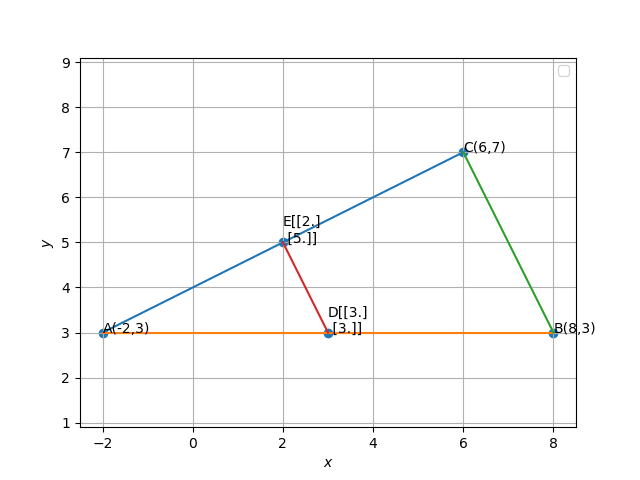
\includegraphics[width=0.55\linewidth]{img.png}
\end{figure}


Consider a triangle $\Delta \vec{ABC}$.
Let $\vec{D}$ and $\vec{E}$ are midpoints on the sides opposite to $\vec{C}$ and $\vec{B}$.
So,
\begin{align}
		\vec{D} = \frac{\vec{A} +\vec{B}}{2}, 
		\vec{E} = \frac{\vec{A} +\vec{C}}{2}
\end{align}
so the line joining the midpoints is
\begin{align}
		\vec{D} - \vec{E} =\frac{\vec{A} +\vec{B}}{2}-\frac{\vec{A} +\vec{C}}{2}
		=\frac{\vec{B} -\vec{C}}{2}
		=\frac{1}{2}\brak{\vec{B} -\vec{C}}= \lambda\brak{\vec{B} -\vec{C}}
\end{align}
So, the line is parallel to the third side as it $\lambda\brak{\vec{B} -\vec{C}}$.

Hence, proved.

\end{document}




